\section{Grundlagen}

\subsection{Der Software Life Cycle}

Abbildung \ref{fig:softwareentwicklungsprozess} zeigt den gesamten Lebenszyklus eines Softwareprodukts. Dieser 
reicht von der Planung inklusive Anforderungsfindung über die Programmierung, bis
hin zum Testen und Betrieb der Software.
Dieser Lebenszyklus ist für jede Software gleich, allerdings unterscheidet sich der
zeitliche und organisatorische Ablauf der Phasen zwischen verschiedenen Vorgehensmodellen
stark \cite{DietmarAbts2017}.

\begin{figure}[H]
    \centering
    \caption{Übersicht des Softwarelebenszyklus}
	\label{fig:softwareentwicklungsprozess}
    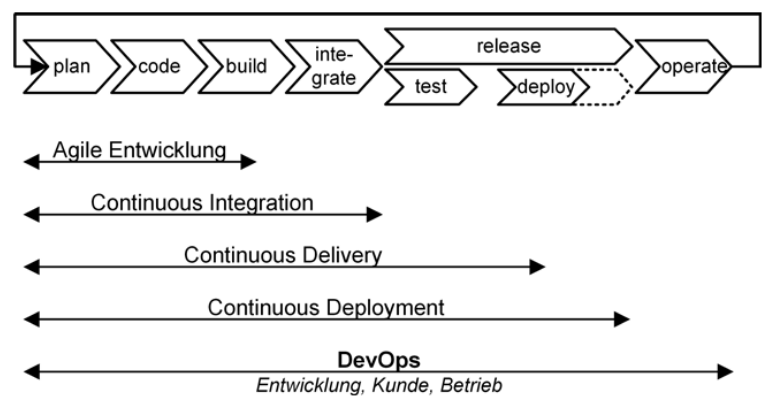
\includegraphics[width=0.8\textwidth]{softwareentwicklungsprozess.png}
    \\
    Quelle: \cite{Halstenberg2020}
\end{figure}

Hier werden die einzelnen Phasen kurz erläutert:

\textbf{Plan}: In dieser Phase wird der Ist-Zustand analysiert und die funktionalen Anforderungen
des Kunden an die Software gesammelt \cite{Halstenberg2020}.

\textbf{Code}: Hier werden die spezifizierten Anforderungen im Code umgesetzt, was
die Hauptaktivität des Entwicklungszyklus darstellt \cite{Halstenberg2020}.

\textbf{Build}: Dies beinhaltet das kompilieren des Programms nach einer Änderung
am Code. Das Ergebnis ist ein ausführbares Programm, welches getestet werden kann.
In einigen interpretierten Programmiersprachen entfällt dieser Schritt \cite{Halstenberg2020}.

\textbf{Integrate}: Hier wird die Software in andere Teile des Gesamtsystems integriert.
Dieser Schritt ist etwas variabel, da viele Abhängigkeiten bereits während des Buildprozesses
integriert werden, manche andere Systeme aber auch erst nach dem Testen der elementaren
Funktionen der Software hinzukommen \cite{Halstenberg2020}.

\textbf{Test}: Beim Testing wird die funktionalität der Software geprüft.
Hier kommen zum einen Unit Tests zum Einsatz, die elementare Funktionen der Software überprüfen,
zum anderen Integration Tests, die die Software im Zusammenhang mit anderen Systemen testen \cite{Halstenberg2020}.

\textbf{Deploy}: In diesem Schritt wird die fertig getestete Software in die Produktionsumgebung
ausgeliefert. Hier kann sie der Kunde nutzen \cite{Halstenberg2020}.

\textbf{Operate}: Im Betrieb wird sichergestellt, dass die Software ordnungsgemäß läuft.
Die Produktionsumgebung wird überwacht um mögliche Fehler zu finden und Nutzungsmetriken werden
erhoben \cite{Halstenberg2020}.

\subsection{Das Wasserfallmodell}

Ein gutes Beispiel für ein Modell der konventionellen Softwareentwicklung ist
das Wasserfallmodell. Die einzelnen Phasen weichen hier leicht von den oben genannten
ab, allerdings ist die Reihenfolge der Schritte in etwa gleich, sie werden lediglich
anders gruppiert \cite{DietmarAbts2017}. Das Modell wird in Abbildung \ref{fig:wasserfall} dargestellt.
Im Kontrast zu agilen Methoden, die nachfolgend vorgestellt werden, werden in diesem
Modell die einzelnen Phasen streng sequentiell durchlaufen. Am Ende jeder Phase werden 
zuvor festgelegte Meilensteine geprüft. Sind diese erreicht, schreitet das gesamte Projekt
in die nächste Phase weiter. Sind die Anforderungen nicht erfüllt, wird die Phase mit leicht
Veränderter Methodik wiederholt \cite{DietmarAbts2017}.
Ein Vorteile dieses Modells sind die Einfachheit und die klare Nachvollziehbarkeit
des Projektstandes.
Die Nachteile sind dagegen vielfältig. So werden Fehler in den frühen Phasen erst sehr
spät entdeckt. Zusätzliche und neue Anforderungen können nicht mehr berücksichtigt werden
und ein Kunde bekommt die Anwendung erst zu sehen, wenn das Projekt komplett ageschlossen ist.
Diese Einschränkungen machen das Vorgehen sehr unflexibel \cite{DietmarAbts2017}.

\begin{figure}[H]
    \centering
    \caption{Das Wasserfallmodell}
	\label{fig:wasserfall}
    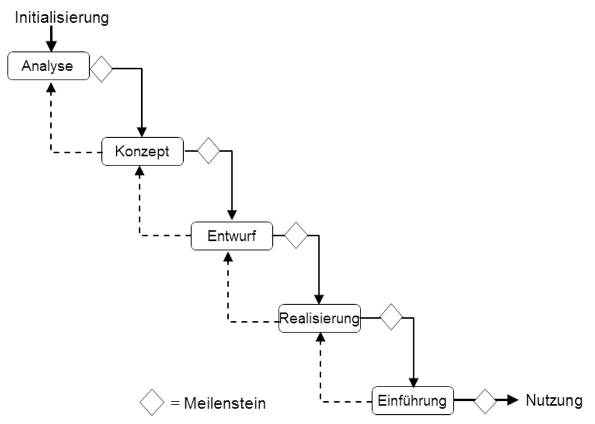
\includegraphics[width=0.8\textwidth]{wasserfall.png}
    \\
    Quelle: \cite{DietmarAbts2017}
\end{figure}

\subsection{Agile Vorgehensmethoden}

Die agile Softwareentwicklung steht in starkem Kontrast zu konventionellen Methoden.
Ziel ist es, den Entwicklungsprozess schlanker zu machen und unnötigen Aufwand zu
reduzieren. Dem Kunden soll so früh wie Möglich eine funktionierende
Software zur Verfügung stehen \cite{DietmarAbts2017}.

Als Beispiel für agile Entwicklung wird Scrum herangezogen.
Hier werden vereinfacht ausgedrückt kleine Arbeitspakete definiert.
Vor einem ein bis vier Wochen langem Sprint wird definiert, welche Arbeitspakete
erledigt werden. Am Ende des Sprints sind diese bereit für die Auslieferung und
es kann im Nächsten Sprint mit dem Umsetzen neuer Anforderungen begonnen werden.
Dies ist ein iterativ-inkrementelles Verfahren, bei dem Anforderungen nach und nach,
anstatt auf einmal umgesetzt werden \cite{DietmarAbts2017}.
Abbildung \ref{fig:scrum} zeigt eine grobe Darstellung des Scrum-Ablaufs.

\begin{figure}[H]
    \centering
    \caption{Darstellung des Scrum Ablaufs }
	\label{fig:scrum}
    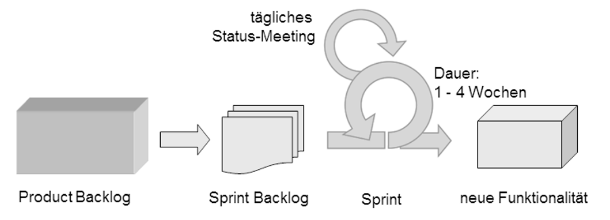
\includegraphics[width=0.8\textwidth]{scrum.png}
    \\
    Quelle: \cite{DietmarAbts2017}
\end{figure}

Diese Vorgehensweise ermöglicht schnellere Auslieferung der Software.
Dadurch kann schnell Feedback vom Kunden eingeholt und Anpassungen vorgenommen werden
was die Qualität der Software verbessert und große Fehler vermeidet \cite{DietmarAbts2017}.
Es ist insgesamt ein wesentlich flexibleres System.